\documentclass[]{exam}
\input{global}
\input{problem-sets}


\setrandomizerseed{1}

% \firstpageheader{{Name:\enspace\makebox[6cm]{\hrulefill}}\\{Physics}}{}{Test on Unit 6:\\Conservation in Mechanical Systems}
\firstpageheader{\textbf{DO NOT WRITE ON THIS DOCUMENT}\\ Version: B}{}{Test on Unit 6:\\Conservation in Mechanical Systems}
\runningheader{Physics}{}{Test on Unit 8: Conservation in Mechanical Systems}


\begin{document}
\begin{questions}

\question
Describe what happens to the energy of the car-earth system as the car moves down the ramp from point A to point B. Assume friction is negligible. 

\begin{center}
    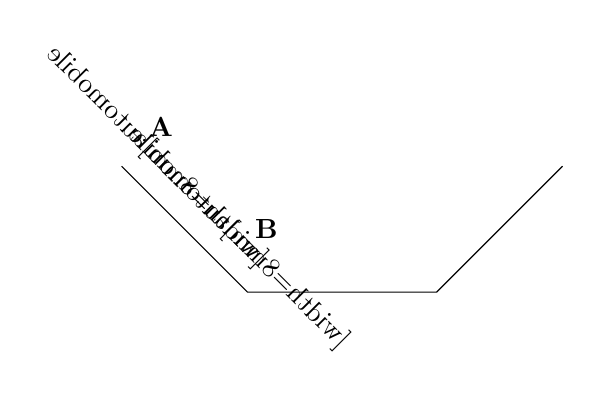
\begin{tikzpicture}[scale=0.8]
        \draw (0,0) -- (2,-2) -- ++(3,0) -- ++(2,2);
        \node[rotate=-45,shift={(0,4mm)}] at (0.2,-0.2) {\reflectbox{\twemoji[width=8mm]{automobile}}} node[shift={(0.5,0.5)}] {\textbf{A}};
        \node[rotate=-45,shift={(0,4mm)}] at (1.5,-1.5) {\reflectbox{\twemoji[width=8mm]{automobile}}}; 
        \node at (2.3,-1) {\textbf{B}};
    \end{tikzpicture}
\end{center}

\begin{randomizechoices}[norandomize]
    \choice The car's kinetic energy stays the same, gravitational potential energy increases, and total energy increases.
    \choice The car's kinetic energy increases, gravitational potential energy increases, and total energy stays the same.
    \choice The car's kinetic energy stays the same, gravitational potential energy stays the same, and total energy stays the same.
    \correctchoice The car's kinetic energy increases, gravitational potential energy decreases, and total energy stays the same.
\end{randomizechoices}

\question
A skater starts at the top of a ramp,  skates down the ramp, and reaches the other side. Which energy bar graph best represents the energy of the skater-earth system when the skater is halfway down the ramp? Assume friction is negligible.



\begin{minipage}{0.6\textwidth}
\centering
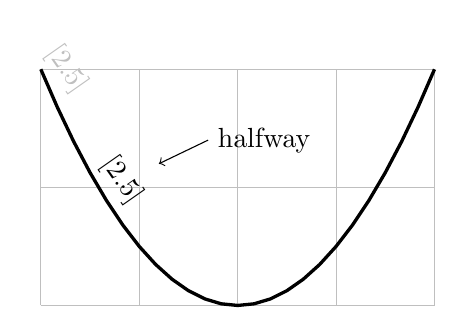
\begin{tikzpicture}[x=2.5cm,y=3cm]
    \draw[step=0.5,lightgray] (-1,0) grid (1,1);
    \draw[very thick, domain=-1:1] plot (\x, {\x*\x});
    \node[rotate=-55,lightgray] at (-0.87,1) {\Strichmaxerl[2.5]};
    \node[rotate=-55] at (-0.59,0.53) {\Strichmaxerl[2.5]};
    \draw[<-] (-0.4,0.6) -- ++(0.25,0.1) node[right] {halfway};
\end{tikzpicture}
\end{minipage}%
\begin{minipage}{0.35\textwidth}
    \centering
    \begin{randomizechoices}[norandomize]
        \choice Graph A
        \correctchoice Graph B
        \choice Graph C
        \choice Graph D
    \end{randomizechoices}    
\end{minipage}%

\bigskip

\begin{center}
    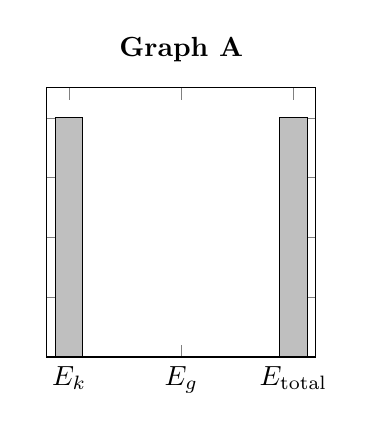
\begin{tikzpicture}
    \begin{axis}[width=5cm,height=5cm,ymin=0,ymax=90,title=\textbf{Graph A},
        symbolic x coords={$E_k$,$E_g$,$E_\mathrm{total}$},
        xtick=data,
        yticklabel=\empty]
        \addplot[ybar,fill=lightgray] coordinates {
            ($E_k$,80)
            ($E_g$,0)
            ($E_\mathrm{total}$,80)
        };
    \end{axis}
    \end{tikzpicture}%
    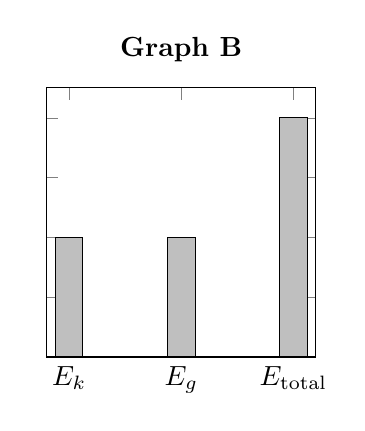
\begin{tikzpicture}
    \begin{axis}[width=5cm,height=5cm,ymin=0,ymax=90,title=\textbf{Graph B},
        symbolic x coords={$E_k$,$E_g$,$E_\mathrm{total}$},
        xtick=data,
        yticklabel=\empty]
        \addplot[ybar,fill=lightgray] coordinates {
            ($E_k$,40)
            ($E_g$,40)
            ($E_\mathrm{total}$,80)
        };
    \end{axis}
    \end{tikzpicture}%
    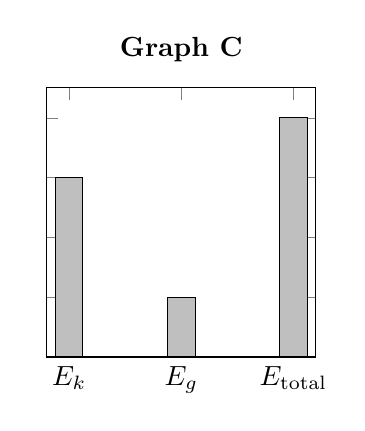
\begin{tikzpicture}
    \begin{axis}[width=5cm,height=5cm,ymin=0,ymax=90,title=\textbf{Graph C},
        symbolic x coords={$E_k$,$E_g$,$E_\mathrm{total}$},
        xtick=data,
        yticklabel=\empty]
        \addplot[ybar,fill=lightgray] coordinates {
            ($E_k$,60)
            ($E_g$,20)
            ($E_\mathrm{total}$,80)
        };
    \end{axis}
    \end{tikzpicture}%
    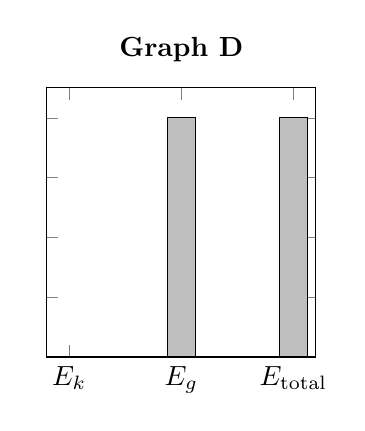
\begin{tikzpicture}
    \begin{axis}[width=5cm,height=5cm,ymin=0,ymax=90,title=\textbf{Graph D},
        symbolic x coords={$E_k$,$E_g$,$E_\mathrm{total}$},
        xtick=data,
        yticklabel=\empty]
        \addplot[ybar,fill=lightgray] coordinates {
            ($E_k$,0)
            ($E_g$,80)
            ($E_\mathrm{total}$,80)
        };
    \end{axis}
    \end{tikzpicture}
\end{center}

\clearpage

\question
A 5-kg box falls off the edge of a 30-meter tall building. How much kinetic energy will the box have right before hitting the ground? Assume air resistance is negligible.


\begin{minipage}{0.3\textwidth}
    \centering
    \begin{randomizechoices}[norandomize]
        \choice \SI{4500}{J}
        \correctchoice \SI{1500}{J}
        \choice \SI{150}{J}
        \choice \SI{750}{J}
    \end{randomizechoices}
\end{minipage}%
\begin{minipage}{0.4\textwidth}
\centering
\begin{tikzpicture}
    \draw[<->,densely dashed] (0,0) -- (0,3) node[pos=0.5,fill=white] {\SI{30}{m}};
    \fill (0,3.15) circle (0.15) node[right=0.15] {\SI{5.0}{kg}};
    \draw[densely dashed] (-2,0) -- (2,0) node[below,pos=0.5] {zero line};
\end{tikzpicture}
\end{minipage}

\question
You drop a \SI{5}{kg} bowling ball from \SI{4}{meters} above a trampoline. When it bounces, it only bounces up \SI{2}{meters}. How much of the ball's energy was removed from the ball-Earth system when the ball after the ball hit the trampoline?

\begin{randomizechoices}[norandomize]
    \choice \SI{200}{J}
    \correctchoice \SI{100}{J}
    \choice \SI{75}{J}
    \choice \SI{50}{J}
\end{randomizechoices}

% \question
% Stickman pushes a \SI{45}{kg} box up a hill. It takes him 10 seconds to reach the top. At the top of the hill, the box has 600 joules of gravitational potential energy. What was Stickman's power output?
% \bigskip

% \begin{minipage}{0.3\textwidth}
%     \begin{randomizechoices}[norandomize]
%         \correctchoice \SI{60}{W}
%         \choice \SI{1200}{W}
%         \choice \SI{20}{W}
%         \choice \SI{240}{W}
%     \end{randomizechoices}
% \end{minipage}%
% \begin{minipage}{0.6\textwidth}
%     \begin{tikzpicture}
%         \draw (0,0) -- (2,2) -- ++(1,0);
%         \begin{scope}[rotate=45]
%             \draw[ultra thick] (0.5,0) rectangle ++(0.5,0.5);
%             \draw[->] (1,0.25) -- ++(0.75,0);
%         \end{scope}
%     \end{tikzpicture}
% \end{minipage}

\question
Dora (\SI{50}{kg}) and Boots (\SI{5}{kg}) are stuck in space.  They drifted away from their spaceship and don’t know how to get back.  In desperation, Dora throws boots \SI{15}{m/s} directly away from the spaceship. What happens to Dora?

\begin{randomizechoices}[norandomize]
    \choice She remains motionless.
    \choice She moves toward the spaceship at \SI{15}{m/s}.
    \correctchoice She moves toward the spaceship at less than \SI{15}{m/s}.
    \choice She moves toward the spaceship at more than \SI{15}{m/s}.
\end{randomizechoices}

\question
A small ball and big ball experience a perfectly \textbf{\underline{inelastic}} collision. The small ball moves at \SI{2.0}{m/s} rightward, toward the big ball. Before the collision, the big ball is at rest. After the collision, the big ball will...

\begin{center}
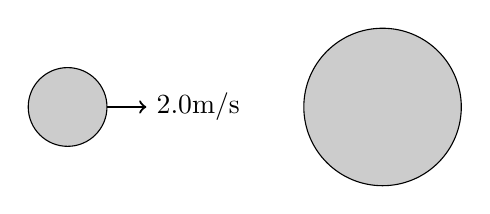
\begin{tikzpicture}
    \draw[thick,->] (0,0) -- (1,0) node[right] {\SI{2.0}{m/s}};
    \draw[fill=black!20] (0,0) circle (0.5);
    \draw[fill=black!20] (4,0) circle (1);
\end{tikzpicture}
\end{center}

\begin{randomizechoices}[norandomize]
    \choice not move at all
    \choice move to the right faster than \SI{2.0}{m/s}
    \correctchoice move to the right slower than \SI{2.0}{m/s}
    \choice move to the left at \SI{2.0}{m/s}
\end{randomizechoices}


\question
A truck is driving down the freeway when it hits a bird. The truck experiences a force of $F$ and a change in momentum of $\Delta p$. If the truck has 1000 times the mass of the bird, what force and change in momentum will the bird experience?

\begin{randomizechoices}[norandomize]
    \choice The bird will experience a force of $1000 F$ and change in momentum of $1000 \Delta p$.
    \choice The bird will experience a force of $1000 F$ and change in momentum of $\Delta p$.
    \choice The bird will experience a force of $F$ and change in momentum of $1000 \Delta p$.
    \correctchoice The bird will experience a force of $F$ and change in momentum of $\Delta p$.
\end{randomizechoices}

\clearpage

\question
An army uses a cannon to shoot a cannonball at a castle's portcullis. 

\begin{center}
\begin{tikzpicture}
    \draw (0,-0.4) rectangle (2.5,0.4) node[above=0.4,pos=0.5] {cannon}; 
    \fill (2.5,0) ellipse (0.12 and 0.4);
    \draw (0.8,-0.1) node {\resizebox{1cm}{!}{\textlinb{\BPwheel}}};
\end{tikzpicture}
\hspace{3cm}
\begin{tikzpicture}
    \draw (0,-0.4) rectangle (2.5,0.4);
    \fill (2.5,0) ellipse (0.12 and 0.4);
    \draw (0.8,-0.1) node {\resizebox{1cm}{!}{\textlinb{\BPwheel}}};
    \draw[->,thick] (-0.1,0) -- ++(-0.5,0);
    \begin{scope}[shift={(3.5,0)}]
        \draw[fill=lightgray] (0,0) circle (0.3) node[above=0.3,shift={(0.1,0)}] {cannonball};
        \draw[->,thick] (0.4,0) -- ++(2.5,0);
    \end{scope}
\end{tikzpicture}
\end{center}

The \SI{1.0}{kg} cannonball leaves the cannon with a velocity of \SI{60}{m/s}. The cannon moves backwards at \SI{2.0}{m/s}. What is the mass of the cannon?

\begin{randomizechoices}[norandomize]
    \choice \SI{1}{kg}
    \choice \SI{50}{kg}
    \choice \SI{120}{kg}
    \correctchoice \SI{30}{kg}
\end{randomizechoices}

\question
Object A is moving with the momentum shown in the momentum vs time graph. Between 4 and 6 seconds, object A has a collision with object B. How much momentum does object B gain during the collision?

\begin{minipage}{0.3\textwidth}
\centering
    \begin{randomizechoices}[norandomize]
        \correctchoice \SI{60}{kg\,m/s}
        \choice \SI{30}{kg\,m/s}
        \choice \SI{100}{kg\,m/s}
        \choice \SI{40}{kg\,m/s}
    \end{randomizechoices}
\end{minipage}%
\begin{minipage}{0.6\textwidth}
\centering
    \begin{tikzpicture}
        \begin{axis}[width=6cm,height=5cm,
            ymin=0,ymax=120,
            xmin=0,xmax=10,
            ylabel={Momentum (\SI{}{kg\cdot m/s})},
            xlabel={Time (s)},
            xtick={0,2,...,10},
            ytick={0,20,...,120},
            axis lines=left,
            grid=both,
            ]
            \draw[thick,rounded corners=1mm] (0,100) -- (4,100) -- (6,40) -- (10,40); 
        \end{axis}
    \end{tikzpicture}
\end{minipage}

% \question
% A \SI{5100}{kg} airplane is flying 1300 meters above the ground. The plane's velocity is \SI{245}{m/s}. Which of the following represents how to calculate the total mechanical energy of the airplane-earth system?

% \begin{randomizechoices}[norandomize]
%     \smallskip
%     \choice $(5100)(10)(1300)\,\text{joules}$\smallskip
%     \choice $ \frac{1}{2}(5100)(245)^2\,\text{joules}$\smallskip
%     \choice $(5100)(10)(1300) - \frac{1}{2}(5100)(245)^2\,\text{joules}$ \smallskip
%     \correctchoice $(5100)(10)(1300) + \frac{1}{2}(5100)(245)^2\,\text{joules}$ \smallskip
% \end{randomizechoices}

\question
Three mountain climbers of equal mass travel up a mountain, but each one takes a different path. Which climber has gained the most gravitational potential energy upon reaching the top of the mountain?

\begin{minipage}{0.5\textwidth}
    \begin{randomizechoices}[norandomize]
        \choice Climber \#1
        \choice Climber \#2
        \choice Climber \#3
        \correctchoice All gravitational potential energies are equal.
    \end{randomizechoices}
\end{minipage}%
\begin{minipage}{0.4\textwidth}
    \centering
    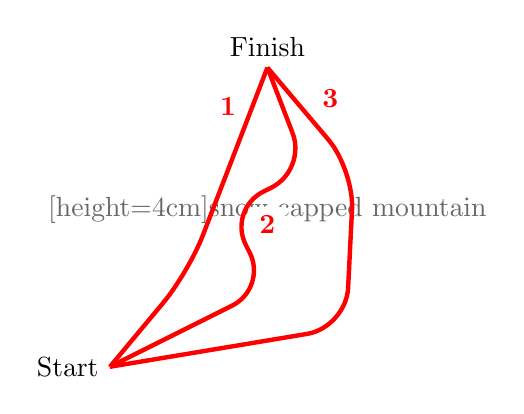
\begin{tikzpicture}
        \coordinate (origin) at (-2,-2);
        \coordinate (peak) at (0,1.8);
        \draw (0,0) node[opacity=0.6] {\twemoji[height=4cm]{snow-capped mountain}};
        \draw[ultra thick,rounded corners=5mm,red] (origin) node[left,black] {Start} -- (-1,-0.8) -- (peak) ;
        \draw[ultra thick,rounded corners=5mm,red] (origin) -- (0,-1) -- (-0.5,0) -- (0.5,0.5)-- (peak);
        \draw[ultra thick,rounded corners=5mm,red] (origin) -- (1,-1.5) -- (1.1,0.5) -- (peak) node[above,black] {Finish};
        \node[red] at (-0.5,1.3) {\textbf{1}};
        \node[red,fill=white] at (0,-0.2) {\textbf{2}};
        \node[red] at (0.8,1.4) {\textbf{3}};
    \end{tikzpicture}
\end{minipage}

% \question 
% You need to lift a heavy weight. How can you increase your power without changing the amount of work you do?

% \begin{randomizechoices}[norandomize]
%     \choice Lift the weight slowly
%     \correctchoice Lift the weight quickly
%     \choice Make the weight lighter
%     \choice Make the weight heavier
% \end{randomizechoices}

% \question
% Two students are asked to move their desks across the room. Student A gets it done it 10 seconds, but student B takes 20 seconds to get it done. What can be said about the power of Student A?

% \begin{randomizechoices}[norandomize]
%     \correctchoice Student A has twice ($2\times$) the power of Student B
%     \choice Student A has quadruple ($4\times$) the power of Student B
%     \choice Student A has half ($1/2\times$) the power of Student B    
% \end{randomizechoices}


\question
A brave monkey stands on the edge of a high-dive diving board.

\begin{center}
\definecolor{clr1}{RGB}{28,163,236}
\definecolor{clr2}{RGB}{35,137,218}
\begin{tikzpicture}
    \fill[clr1] (0,0) rectangle (5,1);
    \draw (0,0) -- (0,3);
    \draw[ultra thick] (0,3) -- (2,3) node[above=-3pt,pos=0.9] {\reflectbox{\twemoji[width=8mm]{monkey}}};
\end{tikzpicture}
\end{center}

The monkey-earth system has \SI{1661}{J} of gravitational potential energy when the monkey is at the top of the board. How much \textbf{\underline{kinetic energy}} does the monkey have at the bottom, right before he lands in the water?

\begin{randomizechoices}[norandomize]
    \correctchoice \SI{1661}{J}
    \choice \SI{-1661}{J}
    \choice \SI{0}{J}
    \choice \SI{760}{J}
\end{randomizechoices}

% \question
% A \SI{4.0}{kg} brick object falls to the ground from a \SI{3.0}{m} tall roof. What is the work done of the brick by the force of gravity?

% \begin{randomizechoices}[norandomize]
%     \choice \SI{0}{J}
%     \choice \SI{40}{J}
%     \correctchoice \SI{120}{J}
%     \choice \SI{12}{J}
% \end{randomizechoices}

\question 
For an object sliding on a surface with friction, what effect does the frictional force have on this system?

\begin{randomizechoices}[norandomize]
    \correctchoice Friction does work to remove energy from the system.
    \choice Friction does not affect the energy of the system.
    \choice Friction does work to add energy to the system.
    \choice There's not enough information given to know the effects of friction on the system.
\end{randomizechoices}

\question
A \SI{5}{kg} book is resting on a shelf that is \SI{2}{m} above the floor. How much gravitational potential energy does the book-earth system have?

\begin{randomizechoices}[norandomize]
    \choice \SI{3}{J}
    \choice \SI{12}{J}
    \choice \SI{70}{J}
    \correctchoice \SI{100}{J}
\end{randomizechoices}




% \question
% A father (\SI{100}{kg}) and his son (\SI{50}{kg}) are jogging at the same speed. The father's kinetic energy is\dots

% \begin{randomizechoices}[norandomize]
%     \correctchoice two times larger than the son's.
%     \choice four times larger than the son's.   
%     \choice two times smaller than the son's.
%     \choice four times smaller than the son's.
% \end{randomizechoices}

% \question
% A \SI{60}{kg} bicyclist is initially at rest. How much energy does the bicycle have after the cyclist does \SI{120}{J} of work on the bicycle through pedaling? (Consider friction negligible).

% \begin{randomizechoices}[norandomize]
%     \choice \SI{2}{J}
%     \choice \SI{4}{J}
%     \choice \SI{60}{J}
%     \correctchoice \SI{120}{J}
% \end{randomizechoices}

\question
The diagram below depicts a 2-kg mass colliding with and sticking to a second box. What is the mass of the second box? Assume friction is negligible.

\begin{center}
    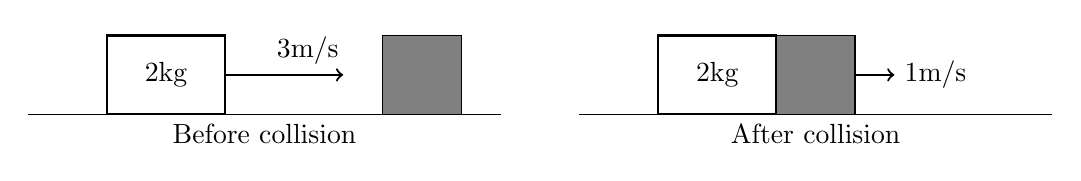
\begin{tikzpicture}
        \draw (0,0) -- (6,0) node[below,pos=0.5] {Before collision};
        \draw[thick] (1,0) rectangle ++(1.5,1) node[pos=0.5] {\SI{2}{kg}};
        \draw[thick,->] (2.5,0.5) -- ++(1.5,0) node[above,pos=0.7] {\SI{3}{m/s}};
        \draw[fill=gray] (4.5,0) rectangle ++(1,1);

        \begin{scope}[xshift=7cm]
            \draw (0,0) -- (6,0) node[below,pos=0.5] {After collision};
            \draw[thick] (1,0) rectangle ++(1.5,1) node[pos=0.5] {\SI{2}{kg}};
            \draw[fill=gray] (2.5,0) rectangle ++(1,1);
            \draw[thick,->] (3.5,0.5) -- ++(0.5,0) node[right] {\SI{1}{m/s}};
        \end{scope}
    \end{tikzpicture}
\end{center}

\begin{randomizechoices}[norandomize]
    \choice \SI{1}{kg}
    \choice \SI{2}{kg}
    \choice \SI{3}{kg}
    \correctchoice \SI{4}{kg}
\end{randomizechoices}


\begin{EnvUplevel}
\textbf{Questions \ref{AtSPK}--\ref{QRwCJ}.} In the diagram shown, a \SI{10}{kg} ball is fired with a velocity of \SI{500}{m/s} from a \SI{1000}{kg} cannon. 
\end{EnvUplevel}

\begin{center}
    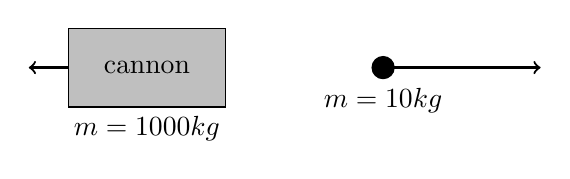
\begin{tikzpicture}
        \draw[fill=lightgray] (0,-0.5) rectangle ++(2,1) node[pos=0.5] {cannon} node[below=0.5cm,pos=0.5] {$m = \SI{1000}{kg}$};
        \draw[thick,->] (0,0) -- ++(-0.5,0);
        \draw[fill] (4,0) circle (4pt) node[below=4pt] {$m = \SI{10}{kg}$};
        \draw[thick,->] (4,0) -- ++(2,0);
    \end{tikzpicture}
\end{center}

\question \label{AtSPK}
What is the momentum of the system before the ball is fired?

\begin{randomizechoices}[norandomize]
    \correctchoice \SI{0}{kg\cdot m/s}
    \choice \SI{1500}{kg\cdot m/s}
    \choice \SI{10}{kg\cdot m/s}
    \choice \SI{5000}{kg\cdot m/s}
\end{randomizechoices}

\question \label{QRwCJ}
What is the momentum of the cannon after the ball is fired? (Assume positive direction is to the right).

\begin{randomizechoices}[norandomize]
    \choice \SI{5000}{kg\,m/s}
    \choice \SI{1000}{kg\,m/s}
    \correctchoice \SI{-5000}{kg\,m/s}
    \choice \SI{-1000}{kg\,m/s}
\end{randomizechoices}

\clearpage

\hrule

\question
In the diagram below, scaled vectors represent the momentum of each of two masses, A and B, sliding toward each other on a frictionless, horizontal surface. Which scaled vector best represents the momentum of the system after the masses collide?

\begin{center}
    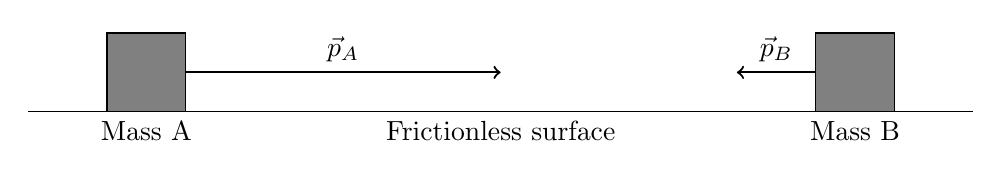
\begin{tikzpicture}
        \draw (0,0) -- (12,0) node[below,pos=0.5] {Frictionless surface};
        \draw[fill=gray] (1,0) rectangle ++(1,1) node[pos=0.5,below=0.5cm] {Mass A} (10,0) rectangle ++(1,1) node[pos=0.5,below=0.5cm] {Mass B};
        \draw[->,thick] (2,0.5) -- ++(4,0) node[above,pos=0.5] {$\vec{p}_\text{\tiny A}$}; 
        \draw[->,thick] (10,0.5) -- ++(-1,0) node[above,pos=0.5] {$\vec{p}_\text{\tiny B}$}; ;
    \end{tikzpicture}
\end{center}

\begin{randomizechoices}[norandomize]
    \choice \tikz{\draw[->,thick] (0,0) -- (-1,0);}
    \correctchoice \tikz{\draw[->,thick] (0,0) -- (+3,0);}
    \choice \tikz{\draw[->,thick] (0,0) -- (-4,0);}
    \choice \tikz{\draw[->,thick] (0,0) -- (+4,0);}
\end{randomizechoices}


\question
The objects below undergo a collision

\begin{center}
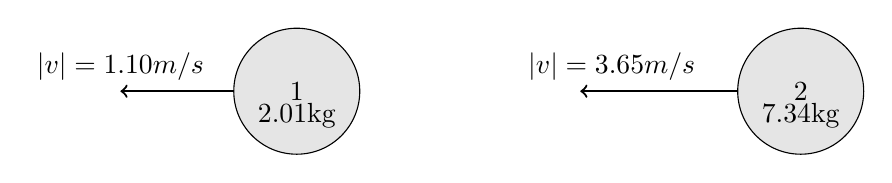
\begin{tikzpicture}[x=8mm,y=8mm]
    \draw[fill=black!10] (0,0) circle (1) node[pos=0.5] {1} node[below=1] {\SI{2.01}{kg}};
    \draw[thick,->] (-1,0) -- ++(-1.8,0) node[above] {$|v| = \SI{1.10}{m/s}$};
    \begin{scope}[shift={(8,0)}]
        \draw[fill=black!10] (0,0) circle (1) node[pos=0.5] {2} node[below=1] {\SI{7.34}{kg}};;
        \draw[thick,->] (-1,0) -- ++(-2.5,0) node[above,pos=0.8] {$|v| = \SI{3.65}{m/s}$};
    \end{scope}
\end{tikzpicture}
\end{center}

If the collision is perfectly \textbf{\underline{inelastic}}, what is the final velocity of the system?

\begin{randomizechoices}
    \correctchoice \SI{-3.10}{m/s}
    \choice \SI{-4.75}{m/s}
    \choice \SI{2.30}{m/s}
    \choice \SI{4.25}{m/s}
\end{randomizechoices}

\begin{solution}
Conservation of momentum is

\begin{equation*}
    m_1 v_{1i} + m_2 v_{2i} = (m_1 + m_2) v_f
\end{equation*}

Dividing $m_1 + m_2$ gives

\begin{align*}
    v_f &= \frac{m_1 v_{1i} + m_2 v_{2i}}{m_1+m_2} \\[1ex]
    &= \frac{(\SI{2.01}{kg})(\SI{-1.10}{m/s}) + (\SI{7.34}{kg})(\SI{-3.65}{m/s})}{\SI{2.01}{kg} + \SI{7.34}{kg}} \\[1ex]
    & = \boxed{\SI{-3.10}{m/s}}
\end{align*}
\end{solution}

\question
The objects below experience a collision.

\begin{center}
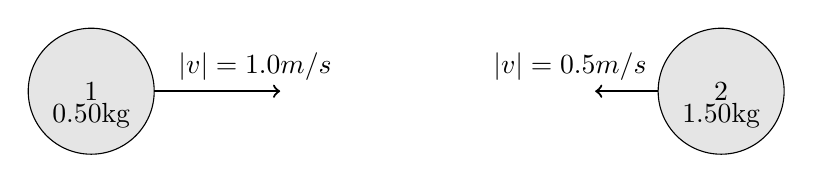
\begin{tikzpicture}[x=8mm,y=8mm]
    \draw[fill=black!10] (0,0) circle (1) node[pos=0.5] {1} node[below=1] {\SI{0.50}{kg}};
    \draw[thick,->] (1,0) -- ++(2,0) node[above,pos=0.8] {$|v| = \SI{1.0}{m/s}$};
    \begin{scope}[shift={(10,0)}]
        \draw[fill=black!10] (0,0) circle (1) node[pos=0.5] {2} node[below=1] {\SI{1.50}{kg}};;
        \draw[thick,->] (-1,0) -- ++(-1,0) node[above,pos=1.4] {$|v| = \SI{0.5}{m/s}$};
    \end{scope}
\end{tikzpicture}
\end{center}

Suppose the collision is \textbf{\underline{elastic}}. Ball 1 recoils at \SI{1.25}{m/s} to the left after the collision. What is the velocity of Ball 2 after they collide?

\begin{randomizechoices}
    \correctchoice \SI{0.25}{m/s}
    \choice \SI{0.50}{m/s}
    \choice \SI{-0.50}{m/s}
    \choice \SI{-0.25}{m/s}
\end{randomizechoices}

\begin{solution}
Conservation of momentum for elastic (hit-and-bounce) collisions is

\begin{equation*}
    m_1 v_{1i} + m_2 v_{2i} = m_1 v_{1f} + m_2 v_{2f}
\end{equation*}

Subtracting $m_1 v_{1f}$ from both sides yields

\begin{equation*}
    m_1 v_{1i} + m_2 v_{2i}  - m_1 v_{1f} = m_2 v_{2f}
\end{equation*}

Diving both sides by $m_2$ leads to

\begin{align*}
    v_{2f} &= \frac{m_1 v_{1i} + m_2 v_{2i}  - m_1 v_{1f}}{m_2} \\[1ex]
    & = \frac{(\SI{0.50}{kg})(\SI{1.0}{m/s}) + (\SI{1.50}{kg})(-\SI{0.50}{m/s}) - (\SI{0.50}{kg})(\SI{-1.25}{m/s})}{\SI{1.50}{kg}} \\[1ex]
    &= \boxed{\SI{0.25}{m/s}}
\end{align*}
\end{solution}

\question
In what type of collision do two colliding objects stick together?

\begin{randomizechoices}
    \correctchoice inelastic
    \choice elastic
    \choice both elastic and inelastic
    \choice neither elastic nor inelastic
\end{randomizechoices}






% \clearpage
% \printkeytable

\end{questions}
\end{document}


\bigskip

\begin{EnvUplevel}
    \centering
    \textbf{PART II. Continued Science Mastery (CSM) Questions}
\end{EnvUplevel}

\question \label{N3JMlC}
In athletics, a ``hammer'' is not construction tool but a 4-kilogram metal ball connected to a handle by a steel wire. Suppose Anita spins the hammer in a circular path, supplying a centripetal force of \SI{320}{N} and giving the hammer a tangential speed of \SI{12}{m/s}. Besides centripetal acceleration and the mass of the hammer, what other information is needed to calculate the centripetal force?


\begin{minipage}{0.4\textwidth}
    \centering
	\begin{randomizechoices}[norandomize]
		\correctchoice radius of curvature
		\choice tangential speed
		\choice Anita's mass
		\choice acceleration due to gravity
	\end{randomizechoices}
\end{minipage}%
\hspace{1cm}
\begin{minipage}{0.6\textwidth}
    \centering
\begin{center}
    \begin{tikzpicture}
        \begin{axis}[
            width=8cm,height=6cm,
            axis line style={draw=none},
            axis equal image,
            ticks=none,
            axis lines=middle,
            xmin=-1.1,xmax=1.6,
            ymin=-0.2,ymax=1.1,
            clip=true,
        ]
        % \clip (-1.1,-0.2) rectangle ++(2.2,1.4);
        \draw[gray,dashed] (0,0) circle (1);
        \begin{scope}[shift={(axis direction cs: 0,-0.05)}]
            \draw[gray,<->] (0,0) -- ({cos(0)},{sin(0)}) node[pos=0.5,below] {$r$};
        \end{scope}
        \draw[Green,very thick,->] ({cos(0)},{sin(0)}) -- ++(axis direction cs: -0.4,0) node[black,above=3pt] {$a_{\text{c}}$};
        \draw[red,very thick,->] ({cos(0)},{sin(0)}) -- ++(axis direction cs: 0,0.7) node[black,pos=1.1] {$\SI{12}{m/s}$};
        \fill (0,0) circle (1pt);
        \fill ({cos(0)},{sin(0)}) circle (3pt) node[right] {$\SI{4.0}{kg}$};
    \end{axis}
    \end{tikzpicture}
    \end{center}
\end{minipage}

\question
A fly tethered by a spider web is undergoing uniform circular motion. At the instant the fly's velocity vector points to the right, what is the direction of the centripetal acceleration?

\begin{minipage}{6cm}
    \centering
    \begin{randomizechoices}[norandomize]
        \correctchoice up
        \choice down
        \choice left
        \choice right
    \end{randomizechoices}
\end{minipage}%
\begin{minipage}{6cm}
    \centering
	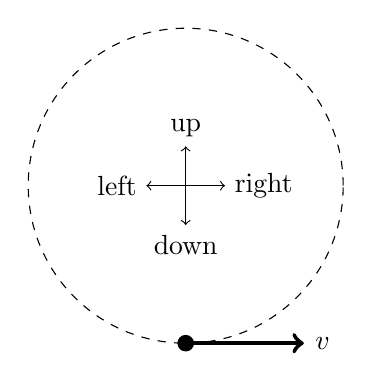
\begin{tikzpicture}
		\draw[dashed] (0,0) circle (2);
		\draw[<->] (0,-0.5) node[below] {down} -- ++(0,1) node[above] {up};
		\draw[<->] (-0.5,0) node[left] {left} -- ++(1,0) node[right] {right};
		\draw[->,ultra thick] (0,-2) -- ++(1.5,0) node[right] {$\bvec{v}$};
		\fill (0,-2) circle (3pt);
	\end{tikzpicture}
\end{minipage}

\clearpage
\question
A tennis ball is launched straight up into the air from the reference point of the ground. At the ball's maximum height, velocity is \fillin[zero].

\begin{randomizechoices}[norandomize]
    \correctchoice zero
    \choice maximum
    \choice increasing
    \choice decreasing
\end{randomizechoices}

\question
After a projectile is launched in the air, in which direction does it experience constant, non-zero acceleration? Ignore air resistance.

\begin{randomizechoices}[norandomize]
	\correctchoice The $y$ direction
	\choice The $x$ direction
	\choice Neither direction
	\choice Both the $x$ and $y$ direction
\end{randomizechoices}

\question
An object on a string is moving around a circle in a counter-clockwise direction as shown below:

\begin{center}
	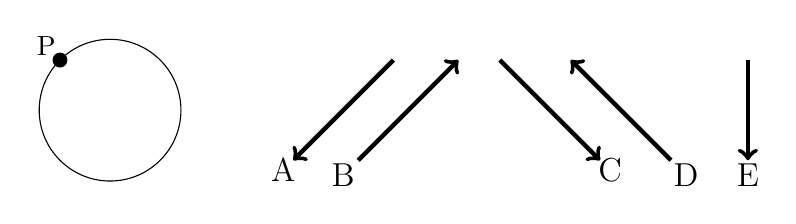
\begin{tikzpicture}[scale=0.9]
		\draw (0,0) circle (1);
		\fill ({-cos(45)},{sin(45)}) circle (3pt) node[above left=-2pt] {P};
		\draw[->,ultra thick] (4,{cos(45)}) -- ++({-2*cos(45)},{-2*sin(45)}) node[pos=1.1] {\large A};
		\draw[->,ultra thick] (3.5,-{cos(45)}) node[below left=-1mm] {\large B} -- ++({2*cos(45)},{2*sin(45)});
		\draw[->,ultra thick] (5.5,{cos(45)}) -- ++({2*cos(45)},{-2*sin(45)}) node[pos=1.1] {\large C};
		\draw[<-,ultra thick] (6.5,{cos(45)}) -- ++({2*cos(45)},{-2*sin(45)}) node[pos=1.15] {\large D};
		\draw[->,ultra thick] (9,{cos(45)}) -- ++(0,{-2*sin(45)}) node[pos=1.15] {\large E};
	\end{tikzpicture}
\end{center}

If the string breaks when the object is at point P, the object will fly off in the direction of which arrow?

\begin{randomizeoneparchoices}[norandomize]
	\correctchoice Arrow A
	\choice Arrow B
	\choice Arrow C
	\choice Arrow D
	\choice Arrow E
\end{randomizeoneparchoices}